\chapter{Конструкторская часть}

\section{Разработка алгоритмов}
На рисунке \ref{scheme:simple} приведена схема стандартного алгоритма перемножения матриц.
На рисунках \ref{scheme:win-top} -- \ref{scheme:fillmul} и \ref{scheme:win-imp-top} -- \ref{scheme:fillmul-imp} приведены
схемы алгоритма Винограда и оптимизированного алгоритма Винограда для перемножения матриц соответственно.

Для алгоритма Винограда худшим случаем являются матрицы нечетной размерности, а лучшим -- четной, поскольку
в таком случае отпадает необходимость в последнем цикле.

Данный алгоритм может быть улучшен путем использования следующих оптимизаций:
\begin{itemize}
	\item использование конструкции a += x вместо a = a + x;
	\item накопление результата в буфер, а затем помещение буфера в ячейку;
	\item замена в циклах k < N/2, k += 1 на k < N, k += 2;
	\item предварительное вычисление констант таких как is\_odd = N \% 2;
	\item замена операции взятия остатка по модулю два (N \% 2) на битовое умножение на 1 (N \& 1);
	\item объединение основного внешнего цикла с последним.
\end{itemize}

\begin{figure}[h]
	\centering
	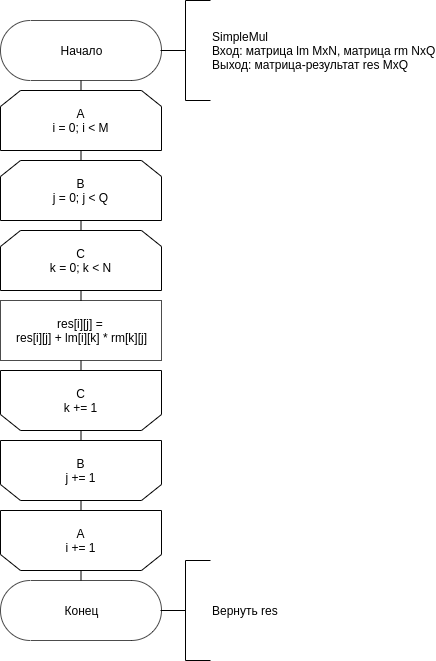
\includegraphics[scale=1]{schemes/simple}
	\caption{Схема стандартного алгоритма перемножения матриц}
	\label{scheme:simple}
\end{figure}

\begin{figure}[h]
	\centering
	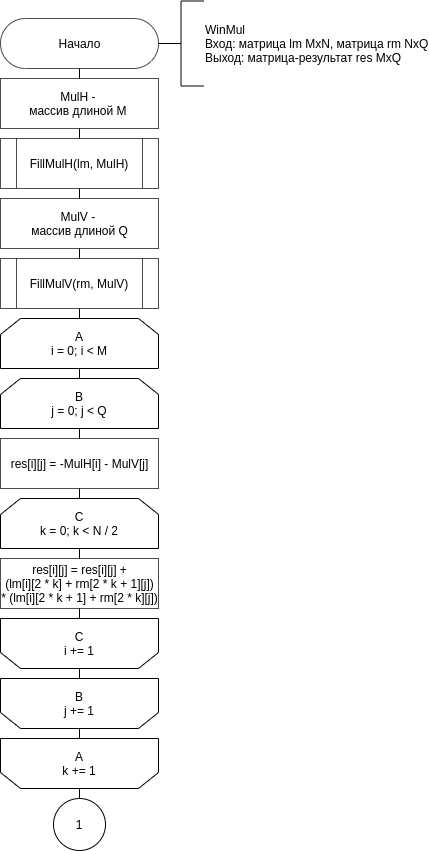
\includegraphics[scale=0.65]{schemes/win-top}
	\caption{Схема алгоритма Винограда для перемножения матриц}
	\label{scheme:win-top}
\end{figure}


\begin{figure}[h]
	\centering
	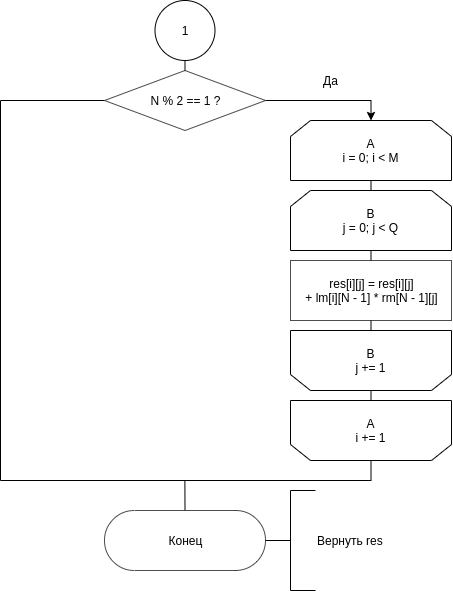
\includegraphics{schemes/win-bottom}
	\caption{Продолжение схемы алгоритма Винограда для перемножения матриц}
	\label{scheme:win-bottom}
\end{figure}


\begin{figure}[h]
	\centering
	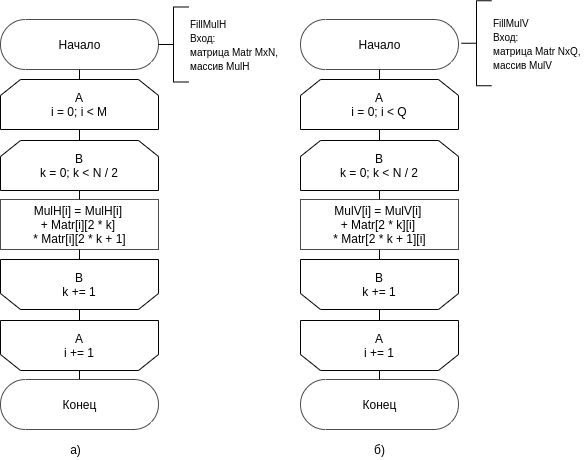
\includegraphics[scale=0.82]{schemes/fillmul}
	\caption{Схема алгоритмов предварительных вычислений в алгоритме Винограда}
	\label{scheme:fillmul}
\end{figure}


\begin{figure}[h]
	\centering
	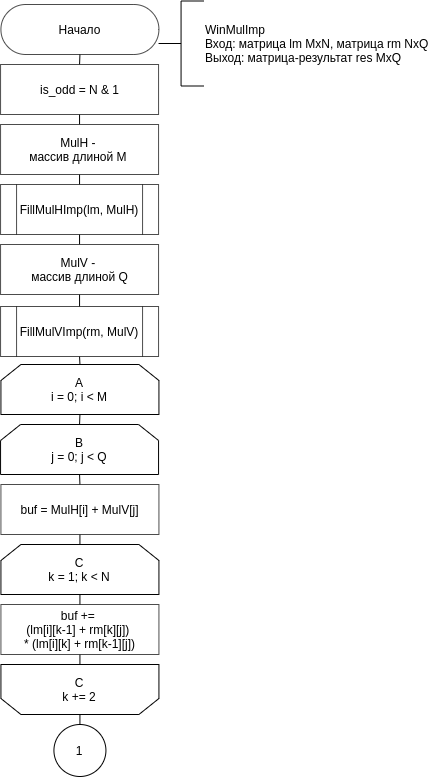
\includegraphics[scale=0.65]{schemes/win-imp-top}
	\caption{Схема оптимизированного алгоритма Винограда для перемножения матриц}
	\label{scheme:win-imp-top}
\end{figure}


\begin{figure}[h]
	\centering
	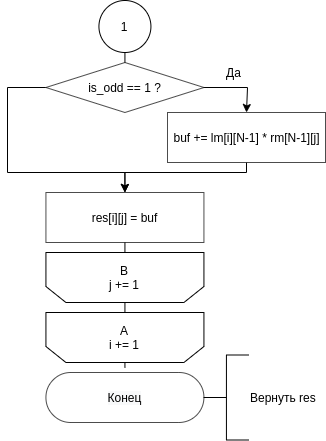
\includegraphics{schemes/win-imp-bottom}
	\caption{Продолжение схемы оптимизированного алгоритма Винограда для перемножения матриц}
	\label{scheme:win-imp-bottom}
\end{figure}



\begin{figure}[h]
	\centering
	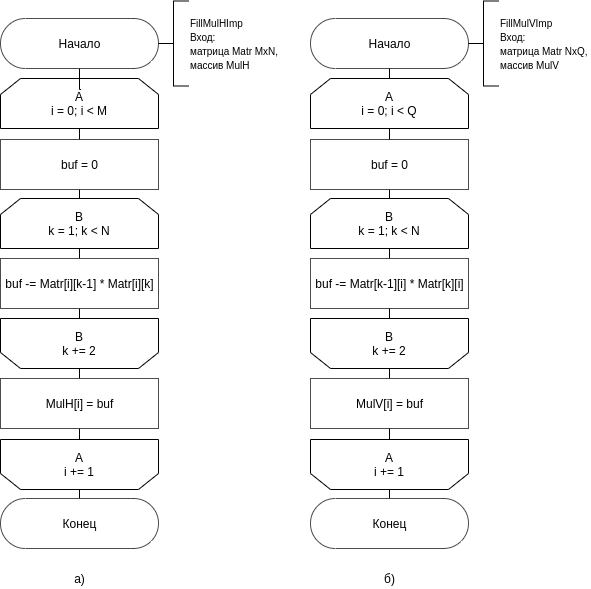
\includegraphics[scale=0.81]{schemes/fillmul-imp}
	\caption{Схема алгоритмов предварительных вычислений в оптимизированном алгоритме Винограда}
	\label{scheme:fillmul-imp}
\end{figure}


\section{Модель вычислений}

Для последующего вычисления трудоемкости введём модель вычислений:

\begin{enumerate}
	\item Трудоемкость базовых операций:
	
	Пусть операции из (\ref{for:opers1}) имеют единичную трудоемкость.
	\begin{equation}
	\label{for:opers1}
	+, -, =, ==, !=, <, >, <=, >=, [], +=, -=, <<, >>
	\end{equation}
	
	Пусть операции из (\ref{for:opers2}) имеют трудоемкость 2.
	\begin{equation}
	\label{for:opers2}
	/, *, \%
	\end{equation}
		
	\item Трудоемкость оператора выбора if условие then A else B рассчитывается, как (\ref{for:if}).
	\begin{equation}
	\label{for:if}
	f_{if} = f_{\text{условия}} +
	\begin{cases}
	f_A, & \text{если условие выполняется,}\\
	f_B, & \text{иначе.}
	\end{cases}
	\end{equation}
	\item Трудоемкость цикла рассчитывается по C-подобной модели, то есть "for (i=0; i<N; i+=1)", как (\ref{for:for}).
	\begin{equation}
	\label{for:for}
	f_{for} = f_{\text{инициализации}} + f_{\text{сравнения}} + N(f_{\text{тела}} + f_{\text{инкремента}} + f_{\text{сравнения}})
	\end{equation}
	\item Трудоемкость вызова функции равна 0.
\end{enumerate}



\section{Трудоемкость алгоритмов}
\subsection{Стандартный алгоритм перемножения матриц}

Трудоёмкость стандартного алгоритма перемножения матриц складывается из трудоемкостей:
\begin{itemize}
	\item Внешнего цикла по $i \in [1..M]$, трудоёмкость которого: $f = 2 + M \cdot (2 + f_{body})$;
	\item Цикла по $j \in [1..Q]$, трудоёмкость которого: $f = 2 + Q \cdot (2 + f_{body})$;
	\item Скалярного умножения двух векторов - цикл по $k \in [1..N]$, трудоёмкость которого: $f = 2 + 11N$;
\end{itemize}

Трудоёмкость стандартного алгоритма равна трудоёмкости внешнего цикла, можно вычислить ее, подставив циклы тела (\ref{for:base}):
\begin{equation}
	\label{for:base}
	f_{base} = 2 + M \cdot (4 + Q \cdot (4 + 11N)) = 2 + 4M + 4MQ + 11MQN \approx 11MQN
\end{equation}

\subsection{Алгоритм Винограда}

Трудоёмкость алгоритма Винограда для перемножения матриц складывается из трудоемкостей:

\begin{enumerate}
	\item Создания векторов $MulH$ и $MulV$ (\ref{for:init}):
	\begin{equation}
	\label{for:init}
	f_{create} = f_{MulH} + f_{MulV};
	\end{equation}
	
	\item Заполнения вектора $MulH$ (\ref{for:MulH}):
	\begin{equation}
	\label{for:MulH}
	f_{MulH}=2+M(2+4+\frac{N}{2}(4+6+2+1+2\cdot3))=\frac{19}{2}MN+6M+2;
	\end{equation}
	
	\item Заполнения вектора $MulV$ (аналогично \ref{for:MulH}):
	\begin{equation}
	\label{for:MulV}
	f_{MulV}=\frac{19}{2}QN+6Q+2;
	\end{equation}
	
	\item Цикла заполнения матрицы для чётных размеров (\ref{for:cycle}):
	\begin{equation}
	\label{for:cycle}
	f_{cycle}=2+M(4+Q(13+\frac{N}{2}\cdot32))=16MNQ+13MQ+4M+2;
	\end{equation}
	
	\item Цикла, для дополнения умножения суммой последних нечётных строки и столбца, если общий размер нечётный (\ref{for:last}):
	\begin{equation}
	\label{for:last}
	f_{last} = 3 + \begin{cases}
	0, & \text{если N - четно}\\
	13MQ+4M+2, & \text{иначе.}
	\end{cases}
	\end{equation}
\end{enumerate}

Cуммарная трудоёмкость:
\begin{equation}
	\label{for:common}
	\begin{split}
		&f_{win-common}=f_{create}+f_{cycle}+f_{last}=16MNQ+13MQ+\frac{19}{2}(MN+QN)+\\
		&+10M+6Q+9+\begin{cases}0 & \text{если N - четно}\\13MQ+4M+2 & \text{иначе.};\end{cases}
	\end{split}
\end{equation}


Итого, для худшего случая (нечётный размер матриц): 
\begin{equation}
	\label{for:worst}
	f_{win-worst\_case} = 16MNQ+26MQ+\frac{19}{2}(MN+QN)+14M+6Q+11;
\end{equation}

Для лучшего случая (чётный размер матриц): 
\begin{equation}
	\label{for:best}
	f_{win-best\_case} = 16MNQ+13MQ+\frac{19}{2}(MN+QN)+10M+6Q+9;
\end{equation}

\subsection{Оптимизированный Алгоритм Винограда}

Трудоёмкость оптимизированного алгоритма Винограда для перемножения матриц складывается из трудоемкостей:

\begin{enumerate}
	\item Создания векторов $MulH$ и $MulV$ (\ref{for:init-imp}):
	\begin{equation}
	\label{for:init-imp}
	f_{create} = f_{MulH} + f_{MulV};
	\end{equation}
	
	\item Заполнения вектора $MulH$ (\ref{for:MulH-imp}):
	\begin{equation}
	\label{for:MulH-imp}
	f_{MulH}=2+M(2+1+2+\frac{N}{2}(2+4+2+1+1)+2)=5MN+7M+2;
	\end{equation}
	
	\item Заполнения вектора $MulV$ (аналогично \ref{for:MulH-imp}):
	\begin{equation}
	\label{for:MulV-imp}
	f_{MulV}=5QN+7Q+2;
	\end{equation}
	
	\item Цикла заполнения матрицы для чётных размеров (\ref{for:cycle-imp}):
	\begin{equation}
	\label{for:cycle-imp}
	\begin{split}
		&f_{cycle}=2+M(4+Q(8+\frac{17N}{2})+4+
		\begin{cases}
			0, & \text{если N - четно}\\
			9, & \text{иначе.}
		\end{cases})=\\
		&=\frac{17}{2}MNQ+MQ\cdot
		\begin{cases}
			12, & \text{если N - четно}\\
			21, & \text{иначе.}
		\end{cases}+4M+2
	\end{split}
	\end{equation}

	\item Определения четности N (\ref{for:odd-check-imp}):
	\begin{equation}
	\label{for:odd-check-imp}
	f_{odd-check} = 2;
	\end{equation}
\end{enumerate}

Cуммарная трудоёмкость:
\begin{equation}
	\label{for:common-imp}
	\begin{split}
		&f_{win\_imp-common}=f_{create}+f_{cycle}+f_{odd-check}=\frac{17}{2}MNQ+5(MN+QN)+\\
		&+9M+7Q+8+\begin{cases}12MQ & \text{если N - четно}\\21MQ & \text{иначе.}\end{cases}
	\end{split}
\end{equation}


Итого, для худшего случая (нечётный размер матриц): 
\begin{equation}
	\label{for:worst-imp}
	f_{win\_imp-worst\_case}=\frac{17}{2}MNQ+5(MN+QN)+21MQ+9М+7Q+8;
\end{equation}

Для лучшего случая (чётный размер матриц): 
\begin{equation}
	\label{for:best-imp}
	f_{win\_imp-best\_case}=\frac{17}{2}MNQ+5(MN+QN)+12MQ+9М+7Q+8;
\end{equation}

\section{Вывод}

В данном разделе были рассмотрены схемы алгоритмов умножения
матриц, введена модель вычисления трудоёмкости, рассчитаны трудоёмкости
алгоритмов. Из формул \ref{for:base}, \ref{for:best}, \ref{for:best-imp} видно, что все три алгоритма имеют зависимость от размерности матриц,
однако оптимизированный алгоритм Винограда имеет наилучший коэффициент перед слагаемым MQN, равный 8, из чего
следует, что он должен быть наиболее эффективным.